\chapter{Summary of Chapter 5: Workflows for Biodiversity Data}
\label{chapter-case-study}

In this chapter we discuss two automated workflows for exchange of biodiversity data developed as part of OpenBiodiv: (1) automatic import of specimen records into manuscripts, and (2) automatic generation of data paper manuscripts from Ecological Metadata Language (EML) metadata. The workflows were presented at a webinar for the orgnization iDigBio\footnote{Integrated Digitized Biocollections (iDigBio) is a US-based aggregator of biocollections data. They hold regular webinars and workshops aimed at improving biodiversity informatics knowledge, which are attended by collection managers, scientists, and IT personnel. Thus, doing a presentation for iDigBio was an excellent way of making the research and tools-development efforts of OpenBiodiv widely known and getting feedback from the community.} and published as a paper (\cite{senderov_online_2016}).

The slides from the presentation as well as a PDF of the paper are available from the webinar GitHub page under \url{https://github.com/vsenderov/idigbio-webinar}.

\section{Introduction}

Information on occurrences of species and information on the specimens that are evidence for these occurrences (specimen records) is stored in different biodiversity databases. These databases expose the information via public REST API's. I focused on the Global Biodiversity Information Facility (GBIF), Barcode of Life Data Systems (BOLD), iDigBio, and PlutoF, and utilized their API's to import occurrence or specimen records directly into a manuscript edited in the ARPHA Writing Tool (AWT).

Furthermore, major ecological and biological databases around the world provide information about their datasets in the form of EML. A workflow was developed for creating data paper manuscripts in AWT from EML files. Such files could be downloaded, for example, from GBIF, DataONE, or the Long-Term Ecological Research Network (LTER Network).

The development of these workflows focuses on two areas: optimizing the workflow of specimen data and optimizing the workflow of dataset metadata. These efforts resulted in the functionality that it is now possible, via a record identifier, to directly import specimen record information from the Global Biodiversity Information Facility (GBIF), Barcode of Life Data Systems (BOLD), iDigBio, or PlutoF into manuscripts in the ARPHA Writing Tool (AWT). No manual copying or retyping is required. 

\section{Presentation}

A video recording of the presentation is available\footnote{\url{http://idigbio.adobeconnect.com/p7sg0aym3e3/}}. More information can be found in the webinar information page\footnote{\url{http://www.idigbio.org/content/online-direct-import-specimen-records-idigbio-infrastructure-taxonomic-manuscripts}}. The slides of the presentation are attached as supplementary files and are deposited in Slideshare\footnote{\url{http://www.slideshare.net/ViktorSenderov/online-direct-import-of-specimen-records-from-idigbio-infrastructure-into-taxonomic-manuscripts}}.

During the presentation we conducted a poll about the occupation of the attendees, the results of which are summarized in Fig.~\ref{fig:webinar-poll}. Of the participants who voted, about a half were scientists, mostly biologists, while the remainder were distributed across IT specialists and librarians, with 20\% "Other." The other categories might have been administrators, decision-makers, non-biology scientists, collections personnel, educators, etc.

\begin{figure}
\centering
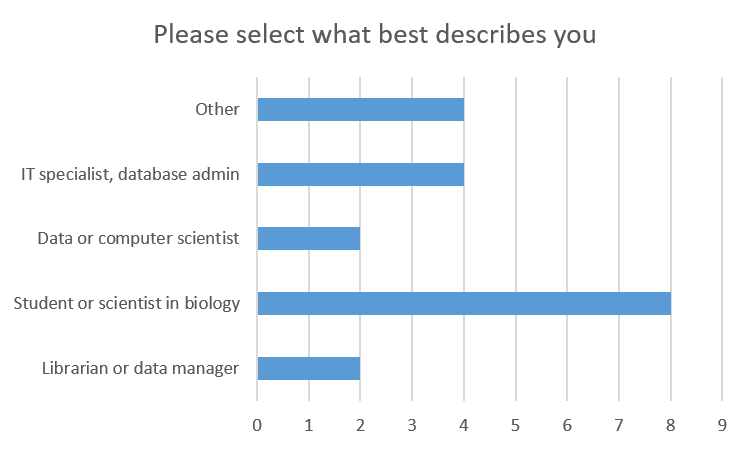
\includegraphics[width=\textwidth]{Figures/webinar-pool}
\decoRule
\caption{Poll results about composition of audience during live participation..}
\label{fig:webinar-poll}
\end{figure}

At the end of the presentation, very interesting questions were raised and discussed. For details, see the ``Results and discussion'' section of this paper.

\section{Methods}

Both workflows discussed  rely on three key standards: RESTful API's for the web (\cite{kurtz_what_2013}), Darwin Core (\cite{wieczorek_darwin_2012}), and EML (\cite{fegraus_maximizing_2005}).

\subsection{Development of workflow 1: Automated specimen record import}

In this subsection we discuss the development of Workflow 1: Automated specimen record import.

\subsection{Development of workflow 2: Automated data paper generation}

In this subsection we discuss the development of Workflow 1: Automated specimen record import.

\section{Results and Discussion}

\subsection{Workflow 1: Automated specimen record import into manuscripts developed in the ARPHA Writing Tool}

It is now possible to directly import a specimen record as a material citation in an ARPHA Taxonomic Paper from GBIF, BOLD, iDigBio, and PlutoF (Slide 5, as well as Fig.~\ref{fig:workflow-idigbio}). The workflow from the user's perspective has been thoroughly described in a blog post; concise stepwise instructions are available via ARPHA's Tips and tricks guidelines. In a nutshell, the process works as follows:

\begin{enumerate}
\item{At one of the supported data portals (BOLD, GBIF, iDigBio, PlutoF), the author locates the specimen record he/she wants to import into the Materials section of a Taxon treatment (available in the Taxonomic Paper manuscript template).}
\item{Depending on the portal, the user finds either the occurrence identfier of the specimen, or a database record identifier of the specimen record, and copies that into the respective upload field of the ARPHA system (Fig.~\ref{fig:occurrence-input-mask}).}
\item{After the user clicks on ``Add,'' a progress bar is displayed, while the specimens are being uploaded as material citations.}
\item{The new material citations are rendered in both human- and machine-readable DwC format in the Materials section of the respective Taxon treatment and can be further edited in AWT, or downloaded from there as a CSV file.}
\end{enumerate}

\begin{figure}
\centering
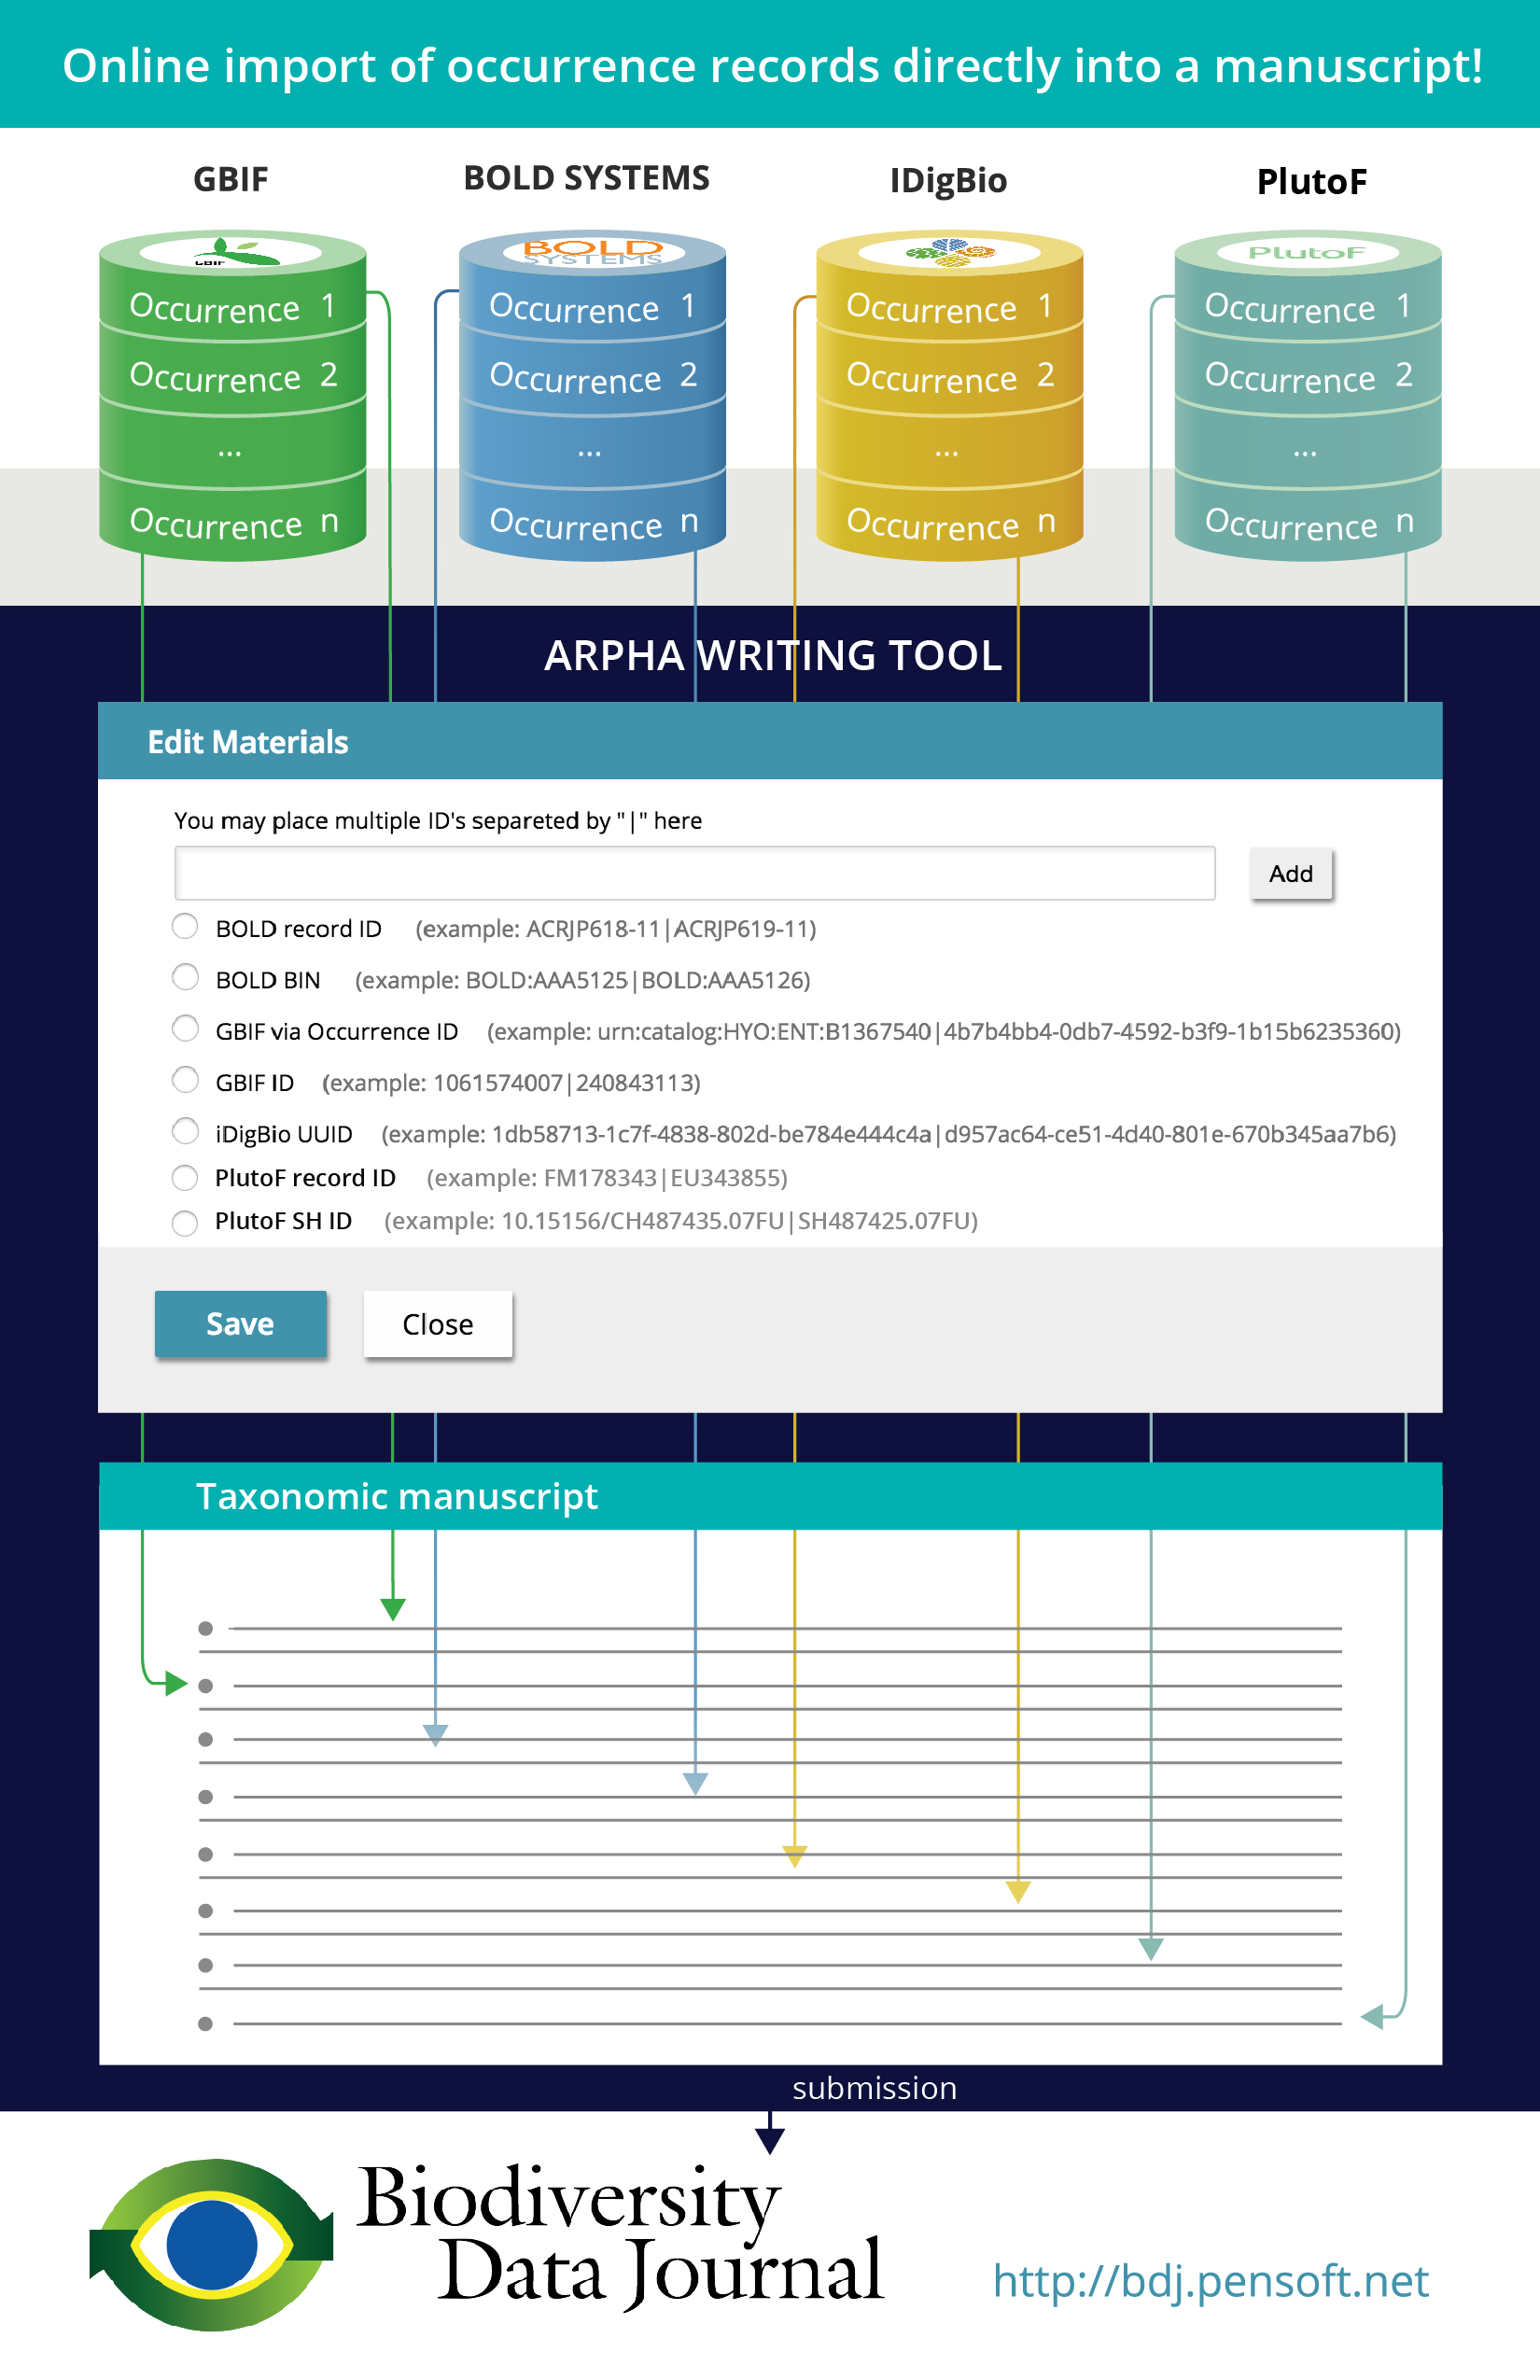
\includegraphics[width=\textwidth]{Figures/workflow-idigbio}
\decoRule
\caption{This fictionalized workflow presents the flow of information content of biodiversity specimens or biodiversity occurrences from the data portals GBIF, BOLD Systems, iDigBio, and PlutoF, through user-interface elements in AWT to textualized content in a Taxonomic Paper manuscript template intended for publication in the Biodiversity Data Journal.}
\label{fig:workflow-idigbio}
\end{figure}

\begin{figure}
\centering
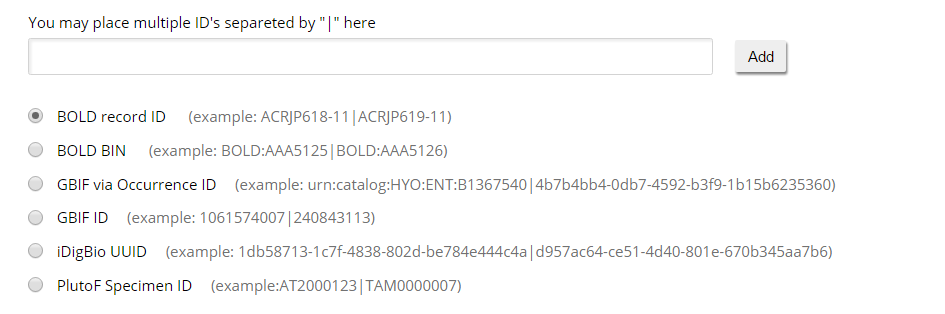
\includegraphics[width=\textwidth]{Figures/occurrence-input-mask}
\decoRule
\caption{User interface of the ARPHA Writing Tool controlling the import of specimen records from external databases.}
\label{fig:occurrence-input-mask}
\end{figure}

\subsubsection{Discussion}

We discuss the availability, or more correctly the lack of persistent unique identifiers (PID's) in the biodiversity informatics space. I furthermore discuss the challenges of importing from our different sources: GBIF, PlutoF, iDigBio, and BOLD. I emphasize how our workflow can be serve as  a curation filter for increasing the quality of specimen data via the scientific peer review process. 

\subsection{Workflow 2: Automated data paper manuscript generation from EML metadata in the ARPHA Writing Tool}

We have created a workflow that allows authors to automatically create data paper manuscripts from the metadata stored in EML (Fig.~\ref{fig:EML-download}, Fig.~\ref{fig:journal-selection}, Fig.~\ref{fig:user-interface}).

\begin{figure}
\centering
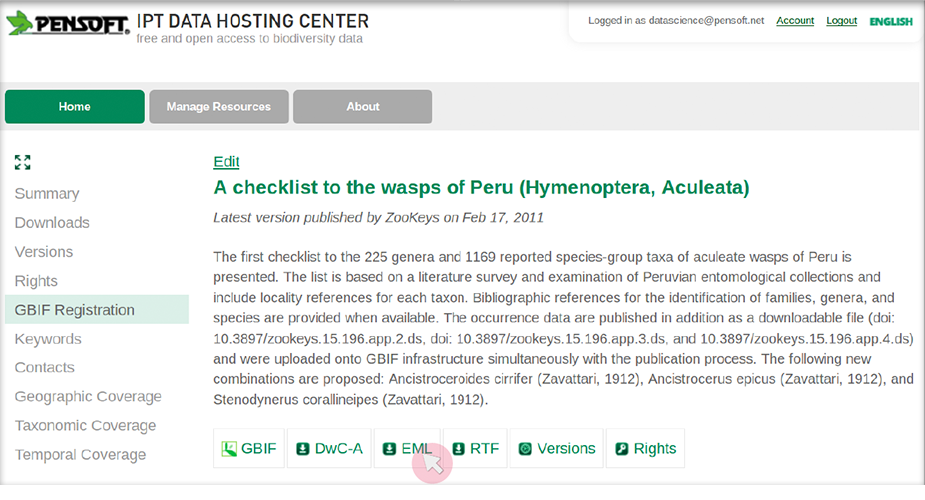
\includegraphics[width=\textwidth]{Figures/EML-download}
\decoRule
\caption{Download of an EML from the GBIF Integarted Publishuing Toolkit (IPT).}
\label{fig:EML-download}
\end{figure}

\begin{figure}
\centering
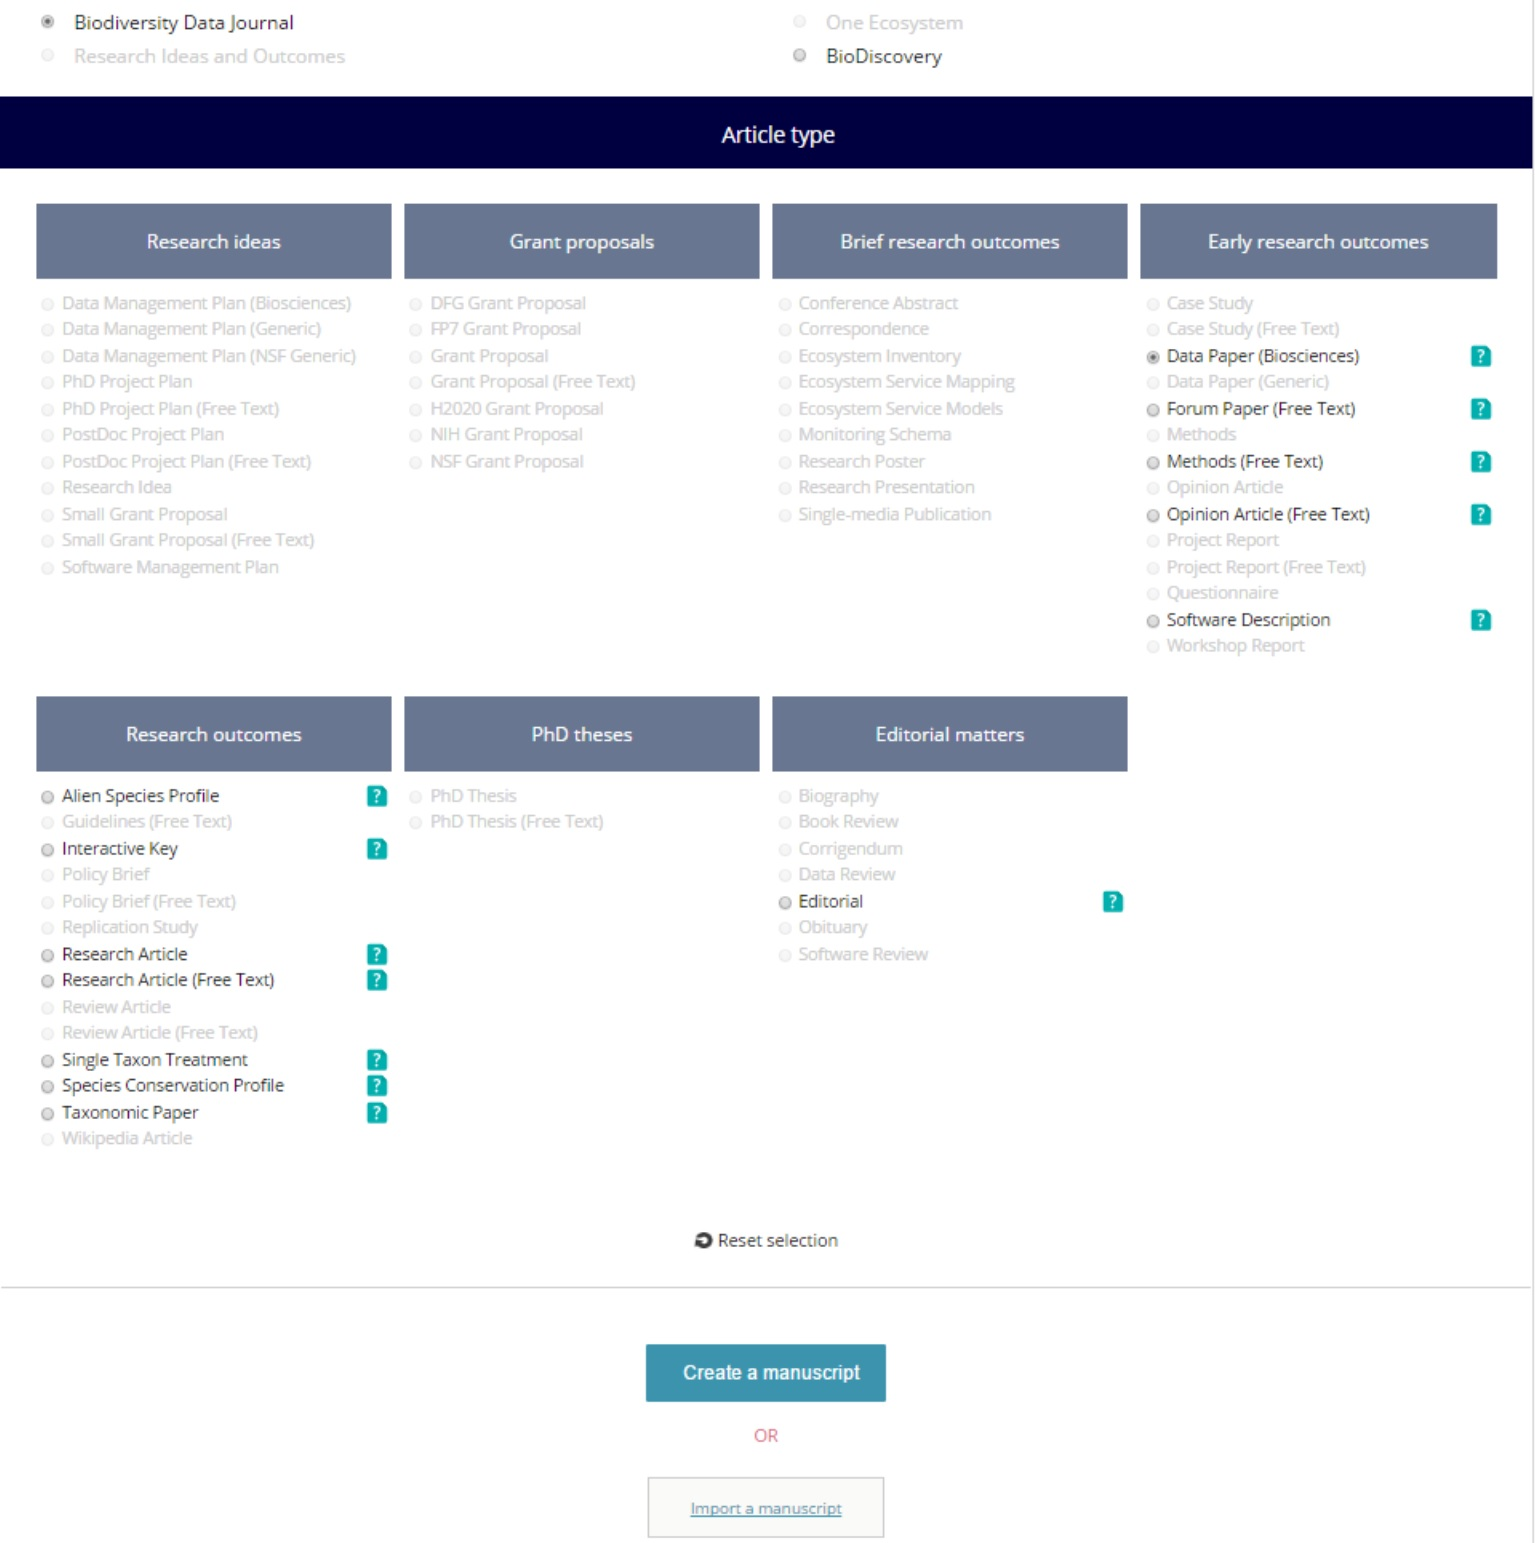
\includegraphics[width=\textwidth]{Figures/journal-selection}
\decoRule
\caption{Selection of the journal and ``Data Paper (Biosciences)'' template in the ARPHA Writing Tool.}
\label{fig:journal-selection}
\end{figure}

\begin{figure}
\centering
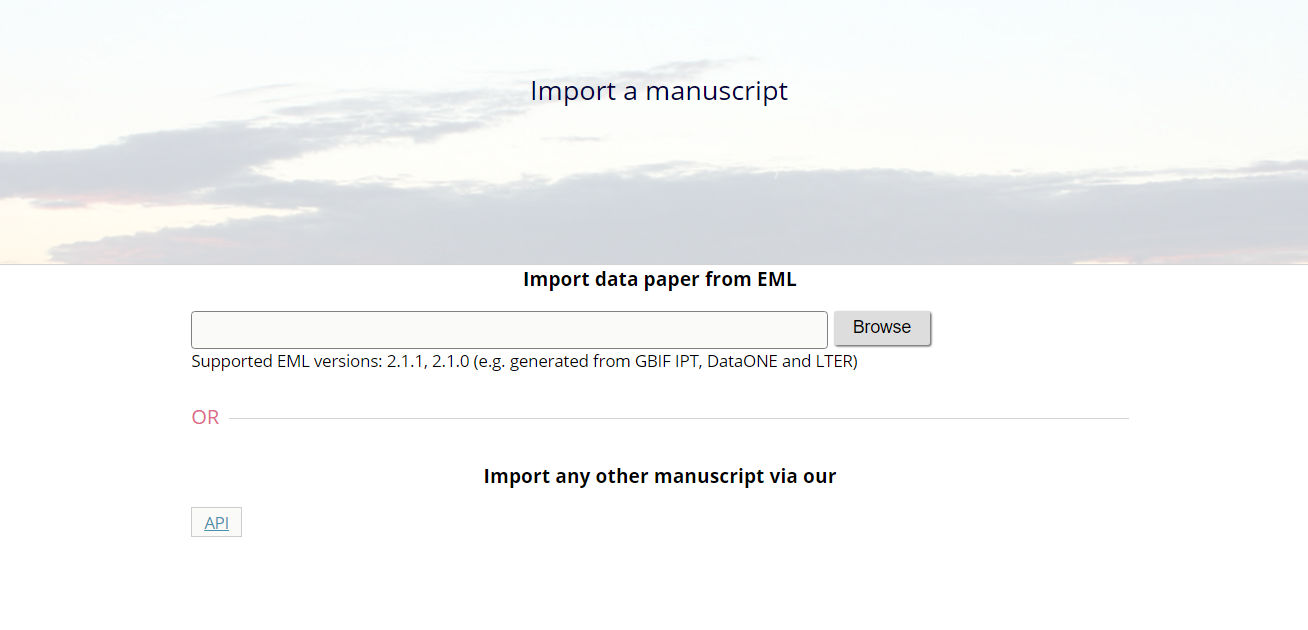
\includegraphics[width=\textwidth]{Figures/user-interface}
\decoRule
\caption{The user interface field for uploading EML files into ARPHA.}
\label{fig:user-interface}
\end{figure}

\subsubsection{Discussion}

I discuss the history of data papers and how our implementation greatly improves the availability of data papers to science practicioners. The two workflows presented generated a lively discussion at the end of the presentation, which is summarized in the Chapter.